\documentclass[14pt]{extbook}
\usepackage{multicol, enumerate, enumitem, hyperref, color, soul, setspace, parskip, fancyhdr} %General Packages
\usepackage{amssymb, amsthm, amsmath, latexsym, units, mathtools} %Math Packages
\everymath{\displaystyle} %All math in Display Style
% Packages with additional options
\usepackage[headsep=0.5cm,headheight=12pt, left=1 in,right= 1 in,top= 1 in,bottom= 1 in]{geometry}
\usepackage[usenames,dvipsnames]{xcolor}
\usepackage{dashrule}  % Package to use the command below to create lines between items
\newcommand{\litem}[1]{\item#1\hspace*{-1cm}\rule{\textwidth}{0.4pt}}
\pagestyle{fancy}
\lhead{Module2}
\chead{}
\rhead{Version B}
\lfoot{6664-2254}
\cfoot{}
\rfoot{test}
\begin{document}

\begin{enumerate}
\item{
First, find the equation of the line containing the two points below. Then, write the equation in the form $ y=mx+b $.\[ (-2, 2) \text{ and } (-8, 7) \]} \newpage
\item{
Find the equation of the line described below. Write the linear equation in the form $y=mx+b$.\[ \text{Parallel to } 5 x + 6 y = 11 \text{ and passing through the point } (2, -10). \]} \newpage
\item{
Solve the equation below.\[ -10(-6x -11) = -3(9x -13) \]} \newpage
\item{
First, find the equation of the line containing the two points below. Then, write the equation in the form $ y=mx+b $.\[ (-5, 9) \text{ and } (10, -10) \]} \newpage
\item{
Solve the equation below.\[ -19(-13x -9) = -17(-8x -14) \]} \newpage
\item{
Solve the linear equation below.\[ \frac{3x -9}{4} - \frac{-7x -3}{7} = \frac{5x + 8}{5} \]} \newpage
\item{
Write the equation of the line in the graph below in Standard Form $Ax+By=C$.
\begin{center}
    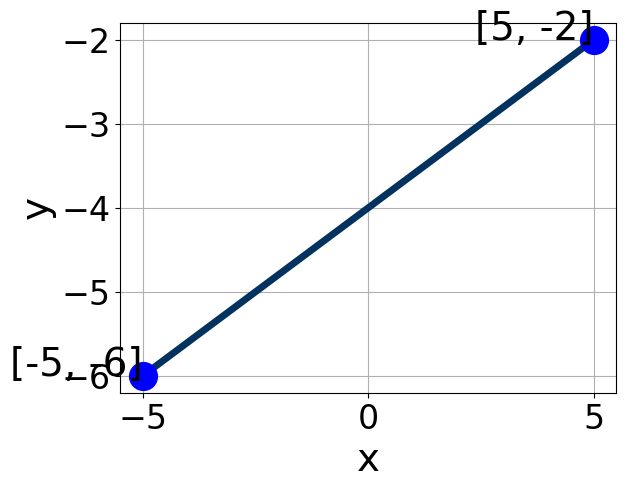
\includegraphics[width=0.5\textwidth]{../Figures/linearGraphToStandardB.png}
\end{center}
} \newpage
\item{
Write the equation of the line in the graph below in Standard Form $Ax+By=C$.
\begin{center}
    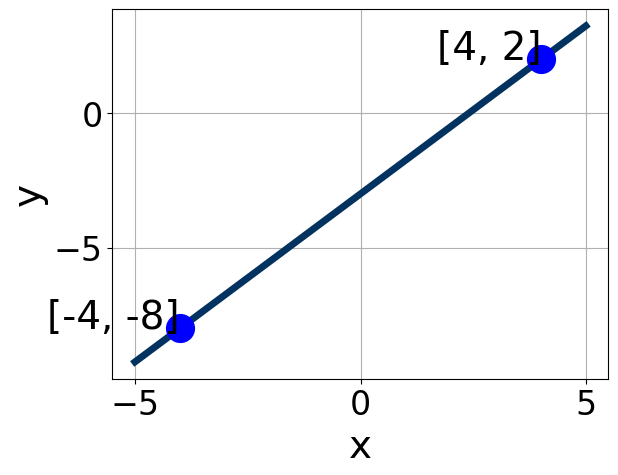
\includegraphics[width=0.5\textwidth]{../Figures/linearGraphToStandardCopyB.png}
\end{center}
} \newpage
\item{
Find the equation of the line described below. Write the linear equation in the form $y=mx+b$.\[ \text{Perpendicular to } 7 x - 5 y = 14 \text{ and passing through the point } (9, 2). \]} \newpage
\item{
Solve the linear equation below.\[ \frac{-4x + 7}{5} - \frac{-6x + 5}{3} = \frac{8x + 7}{6} \]} \newpage
\end{enumerate}

\end{document}